%%%%%%%%%% DOCUMENT STUFF %%%%%%%%%%

\documentclass[10.5pt,letterpaper]{article}
\usepackage{mathtools}
\usepackage{amsmath}
\usepackage{amssymb}
\usepackage{datetime}
\usepackage{setspace}
\usepackage{tikz}
\usepackage[margin=1in]{geometry}
\usepackage{courier}
\usepackage{listings}
\usepackage{mips}
\usepackage{graphicx}
\usepackage{enumitem}
\usepackage{pgfplots}
\usepackage{colortbl}
\usepackage{mdframed}

%%%%%%%%%% FORMATTING %%%%%%%%%%

\newdate{date}{17}{08}{2017}
\spacing{1.5}
\date{\displaydate{date}}
\setcounter{secnumdepth}{0}
\newcommand\tab[1][0.5cm]{\hspace*{#1}}
\newcommand*\circled[1]{\tikz[baseline=(char.base)]{
            \node[shape=circle,draw,inner sep=2pt] (char) {#1};}}
\lstset{language=[mips]Assembler}
\usetikzlibrary{arrows,shapes,automata,petri,positioning,calc}

\tikzset{
    place/.style={
        circle,
        thick,
        draw=black,
        minimum size=6mm,
    },
        state/.style={
        circle,
        thick,
        draw=black!75,
        %fill=blue!20,
        minimum size=6mm,
    },
}

\graphicspath{{images/}}

%%%%%%%%%% CONTENT %%%%%%%%%%

%%%%% COVER PAGE %%%%%

\begin{document}
\title{CS 181: Homework 3}
\author{
	Jonathan Woong\\
	804205763\\
	Summer 2017\\
	Discussion 1A}
\maketitle
\pagebreak

%%%%% PROBLEMS %%%%%

\begin{enumerate}[label=\textbf{Problem \arabic*.}]
\item For each of the following languages
	\begin{enumerate}[label=\roman*)]
		\item \textbf{L$_1$} = $\{a^p;p$ is a prime number\}
		\item \textbf{L$_2$} = $\{a^p;p$ is a prime number, $m$ is a fixed number and $m\geq p\geq 0$\}
		\item \textbf{L$_3$} = $\{a^pb^p;p$ is a prime number\}
		\item \textbf{L$_4$} = $\{a^pb^p;p$ is a prime number, $m$ is a fixed number and $m\geq p\geq 0$\}
		\item \textbf{L$_5$} = $\{a^p;p$ is a prime number and $p$ is a number of a Turing machine $T_p$ that does not halt given the input $p$\}
	\end{enumerate}
	find if it is:
	\begin{enumerate}[label=\alph*)]
		\item a regular language
		\item a context-free language
		\item a recursively enumerable language
	\end{enumerate}
	If the case (a) is true for the language \textbf{L}$_i$, build a finite automaton $A$ such that L($A$)=\textbf{L}$_i$.\\
	If the case (b) is true for the language \textbf{L}$_i$, build a PDA $D$ and formal grammar $G$ such that L($D$)=L($G$)=\textbf{L}$_i$.\\
	If the case (c) is true for the language \textbf{L}$_i$, build a TM $T$ such that L($T$)=\textbf{L}$_i$.\\
	If the case (d) is true for the language \textbf{L}$_i$, build an ITM $M$ such that L($M$)=\textbf{L}$_i$.
	\begin{enumerate}[label=\roman*)]
		\item \textbf{L$_1$} = $\{a^p;p$ is a prime number\}
			Assume \textbf{L$_1$} is context free.\\
			Let $w = a^p$ for some prime number $p \geq k$.\\
			By pumping lemma, we can write $w = uvxyz$. We expect $uv^kxy^kz \in \textbf{L$_1$} \forall k$.\\
			Let $v=a^q$ and $y=a^t$.
			\begin{enumerate}[label=\textbf{Case \arabic*:}]
				\item Let $k = |uxz| = p-q-t$.\\
				Then $|uv^kxy^kz|=k+kq+kt=k(1+q+t).$\\
				$\therefore$ Since the above length is divisible by both $k$ and $(1+q+t)$, it must not be prime. 
				\item Let $k=0$.\\
				Then $|uv^kxy^kz|=|v^2y^2|=2p$.\\
				$\therefore$ Since the above length is divisible by 2, it must not be prime.
				\item Let $k=1$.\\
				Then $|uv^{p+1}xy^{p+1}z|=1+(p+1)q+(p+1)t=1+(p+1)(q+t)=1+(p-1)(p+1)=p^2$.\\
				$\therefore$ Since the above length is the square of $p$, it must not be prime.
			\end{enumerate}
			$\therefore$ By contradiction, \textbf{L$_1$} cannot be a context-free language.
		\item \textbf{L$_2$} = $\{a^p;p$ is a prime number, $m$ is a fixed number and $m\geq p\geq 0$\}\\
			\textbf{L$_2$} is a regular language because we can build an NFA $A$ such that L($A$)= \textbf{L$_2$}.\\
			We construct the NFA with $m$ states, where each prime numbered state is an accepting state, and each non-prime numbered state is not an accepting state. State $m$ is an accepting state if $m=p$.
			\begin{center}
				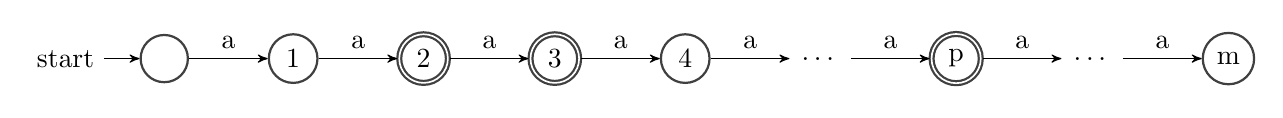
\begin{tikzpicture}[node distance=1cm and 1cm,>=stealth',auto, every place/.style={draw}]
			    \node [state,initial] (0) {};
			    \node [state] (1) [right=of 0] {1};
			    \node [state,accepting] (2) [right=of 1] {2};
			    \node [state,accepting] (3) [right=of 2] {3};
			    \node [state] (4) [right=of 3] {4};
			    \node [state,draw=white] (dot) [right=of 4] {\dots};
			    \node [state,accepting] (p) [right=of dot] {p};
			    \node [state,draw=white] (dot2) [right=of p] {\dots};
			    \node [state] (m) [right=of dot2] {m};
			    \path [->]
			    (0) edge  node {a} (1)
			    (1) edge node {a} (2)
			    (2) edge node {a} (3)
			    (3) edge node {a} (4)
			    (4) edge node {a} (dot)
			    (dot) edge node {a} (p)
			    (p) edge node {a} (dot2)
			    (dot2) edge node {a} (m); 
				\end{tikzpicture}
			\end{center}
		\item \textbf{L$_3$} = $\{a^pb^p;p$ is a prime number\}\\
			Assume \textbf{L$_3$} is a context-free language.\\
			Let $w=a^pb^p$.\\
			Since context-free languages are closed under concatenation, consider the language \textbf{L} = \{$ww^Rw$\}. Assume \textbf{L} is context-free.\\
			Let $ww^Rw=a^pb^{2p}a^{2p}b^p=uvxyz$ where $|vxy|\leq p$, $r=a^pb^{2p}$, $s=a^{2p}b^p$.\\
			The number of $a \in r$ is half the number of $a \in s$.\\
			The number of $b \in r$ is twice the number of $b \in s$.
			\begin{enumerate}[label=\textbf{Case \arabic*:}]
				\item Suppose $v=a \in r$ and $y=a \in s$.\\
				By pumping $|uv^kxy^kz| \forall k$, the number of $a \in r$ will no longer be half the number of $a \in s$, as the quantity of both will be increased by pumping length $k$.\\
				$\therefore$ This case does not satisfy the pumping lemma.
				\item Suppose $v=b \in r$ and $y=b \in s$.\\
				By pumping $|uv^kxy^kz| \forall k$, the number of $b \in r$ will no longer be twice the number of $b \in s$, as the quantity of both will be increased by pumping length $k$.\\
				$\therefore$ This case does not satisfy the pumping lemma.
				\item Suppose $v=ab$ or $y=ab$.\\
				By pumping $|uv^kxy^kz| \forall k$, the word will obtain alternating sequences of $ab$ that do will never be accepted by \textbf{L$_3$}. 
				$\therefore$ This case does not satisfy the pumping lemma.
			\end{enumerate}
			$\therefore$ By contradiction, \textbf{L} cannot be a context-free language. Since \textbf{L} is not a context-free language, \textbf{L$_3$} cannot be a context-free language. 
		\item \textbf{L$_4$} = $\{a^pb^p;p$ is a prime number, $m$ is a fixed number and $m\geq p\geq 0$\}\\
			\textbf{L$_4$} is a regular language because we can build an NFA $A$ such that L($A$)=\textbf{L$_4$}.
			\begin{center}
				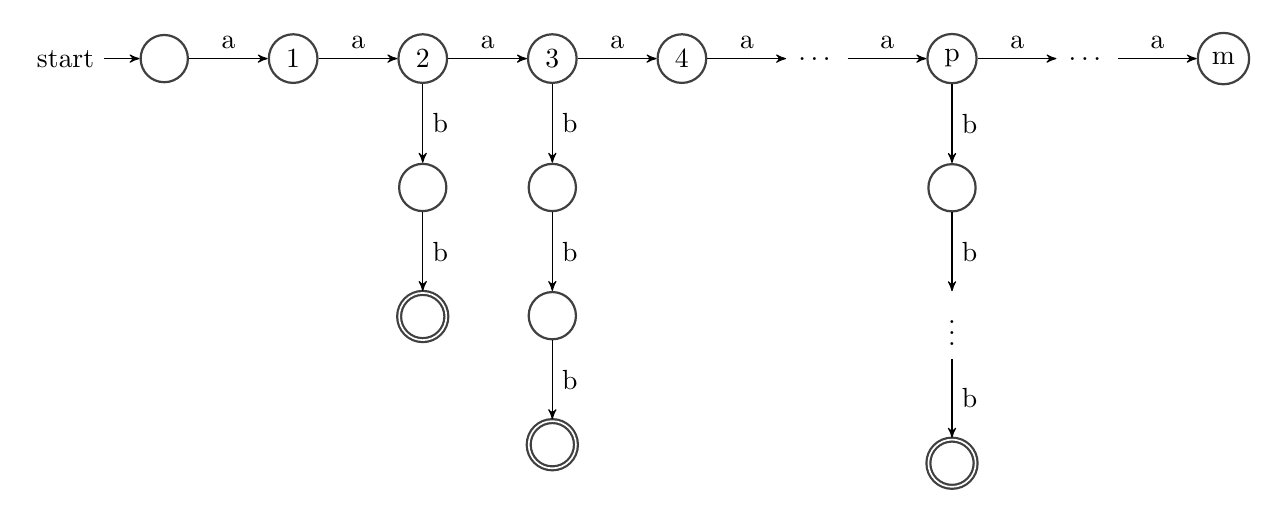
\begin{tikzpicture}[node distance=1cm and 1cm,>=stealth',auto, every place/.style={draw}]
			    \node [state,initial] (0) {};
			    \node [state] (1) [right=of 0] {1};
			    \node [state] (2) [right=of 1] {2};
			    \node [state] (2a) [below=of 2] {};
			    \node [state,accepting] (2b) [below=of 2a] {};
			    \node [state] (3) [right=of 2] {3};
			    \node [state] (3a) [below=of 3] {};
			    \node [state] (3b) [below=of 3a] {};
			    \node [state,accepting] (3c) [below=of 3b] {};
			    \node [state] (4) [right=of 3] {4};
			    \node [state,draw=white] (dot) [right=of 4] {\dots};
			    \node [state] (p) [right=of dot] {p};
			    \node [state] (pa) [below=of p] {};
			    \node [state,draw=white] (pb) [below=of pa] {\vdots};
			    \node [state,accepting] (pc) [below=of pb] {};
			    \node [state,draw=white] (dot2) [right=of p] {\dots};
			    \node [state] (m) [right=of dot2] {m};
			    \path [->]
			    (0) edge  node {a} (1)
			    (1) edge node {a} (2)
			    (2) edge node {a} (3)
			    edge node {b} (2a)
			    (2a) edge node {b} (2b)
			    (3) edge node {a} (4)
			    edge node {b} (3a)
			  	(3a) edge node {b} (3b)
			  	(3b) edge node {b} (3c)
			    (4) edge node {a} (dot)
			    (dot) edge node {a} (p)
			    (p) edge node {a} (dot2)
			    edge node {b} (pa)
			    (pa) edge node {b} (pb)
			    (pb) edge node {b} (pc)
			    (dot2) edge node {a} (m); 
				\end{tikzpicture}
			\end{center}
		\item \textbf{L$_5$} = $\{a^p;p$ is a prime number and $p$ is a number of a Turing machine $T_p$ that does not halt given the input $p$\}
			\textbf{L$_5$} is a recursively enumerable language because we can build a Turing machine $T$ such that L($T$)= \textbf{L$_5$}.\\
			$T$ has tape $A$ and tape $B$. Tape $A$ has the string $a^p$ written on it, for which each $a$ resides in one cell.\\
			$T$ rejects $a^p$ if $p=0$ or $p=1$.\\
			$T$ begins by writing 2 $a$'s from tape $A$ onto tape $B$.\\
			With both heads at the leftmost position, both pointing to the first $a$ of each tape, they advance one cell at a time from left to right.\\
			Once tape $B$ reaches a blank cell, the head for tape $B$ returns to the leftmost position, and both heads continue to advance one cell at a time.\\
			If both tape heads reach a blank at the same time, we know that the length of $a^p$ is divisible by the number of $a$'s in tape $B$. In this case, $T$ adds another $a$ into tape $B$ and repeats the process with both heads starting at the leftmost position.\\
			When both tape heads do not reach a blank at the same time for all lengths of tape $B$, then the length of $a^p$ must be prime. 

\item Let $T_1,T_2,T_3,\dots,T_n,\dots$ be a constructive enumeration of all Turing machines with alphabet \{0,1\} and one linear tape. For each of the following sets
	\begin{enumerate}[label=\roman*)]
		\item \textbf{X}$_1$ = \{$p;p$ is a prime number\}
		\item \textbf{X}$_2$ = \{$px;p$ is a fixed prime number and $x$ is a number of a Turing machine $T_x$ that halts given the input $x$\}
		\item \textbf{X}$_3$ = \{$x;x$ is a number of a Turing machine $T_x$ that does not halt given the input $x$\}
	\end{enumerate}
	find if it is:
	\begin{enumerate}[label=\alph*)]
		\item decidable/recursive
		\item recursively enumerable
		\item inductively decidable
	\end{enumerate}
	\begin{enumerate}[label=\roman*)]
		\item \textbf{X}$_1$ = \{$p;p$ is a prime number\}\\
			\textbf{X}$_1$ is recursively decidable. We can construct a turing machine that implements the Euclidian Algorithm, which correctly identifies prime numbers given the set of all natural numbers.\\
			\textbf{X}$_1$ is also recursively enumerable, since we can construct a turing machine that enumerates over all prime numbers in the set.
		\item \textbf{X}$_2$ = \{$px;p$ is a fixed prime number and $x$ is a number of a Turing machine $T_x$ that halts given the input $x$\}\\
			\textbf{X}$_2$ is recursively enumerable, since an input word $px$ to a turing machine may not halt when $x$ does not exactly match the number of the turing machine. For example, if the input $px$ is given to the turing machine $T_y$ where $x\neq y$, the turing machine $T_y$ may never halt, making \textbf{X}$_2$ a recursively enumerable set.
		\item \textbf{X}$_3$ = \{$x;x$ is a number of a Turing machine $T_x$ that does not halt given the input $x$\}\\
			\textbf{X}$_3$ is inductively decidable, since none of $T_x$ halts when given input. We can build a machine, like in class, with an inductive turing machine $M$. When $x$ is used as input to $M$, it enters an inner machine which outputs the pair $(x,c(T))$ where $c(T)$ is the code of the turing machine. The pair acts as input into a universal turing machine $u$. If $x$ is accepted by $M$, $u$ will output yes. If $x$ is not accepted by $M$, $u$ will output no. Since none of the $T_x$ halts, $u$ will work indefinitely.
	\end{enumerate}
\end{enumerate}
\end{enumerate}
\end{document}